\documentclass[10pt]{beamer}

\usepackage[backend=bibtex,firstinits=true,style=verbose-inote,citestyle=authortitle]{biblatex}
\usepackage{bm}
\usepackage{graphicx}
\usepackage{subcaption}
\usepackage{makecell}
\newcommand{\expect}[2][]{
\ifthenelse{\equal{#1}{}}{
\mathbb{E}\left[#2\right]
}{
\underset{#1}{\mathbb{E}}\left[#2\right]
}}

\newcommand{\cov}[2][]{
\ifthenelse{\equal{#1}{}}{
\text{Cov}\left[#2\right]
}{
\underset{#1}{\text{Cov}}\left[#2\right]
}}


\newcommand{\var}[2][]{
\ifthenelse{\equal{#1}{}}{
\text{Var}[#2]
}{
\underset{#1}{\text{Var}}[#2]
}}

\newcommand{\loss}[2][]{
\ifthenelse{\equal{#1}{}}{
\mathcal{L}(#2)
}{
\mathcal{L}_{#1}(#2)
}}

\newcommand{\kl}[2]{
\text{D}_\text{KL}[#1 \parallel #2]
}

\newcommand{\R}{\mathbb{R}}
%\newcommand{\Prob}{\mathbb{P}}

\newcommand{\1}[1]{\mathds{1}\{#1\}}


%\usecolortheme{dolphin}
\setbeamertemplate{navigation symbols}{}
\setbeamertemplate{section in toc}{\inserttocsectionnumber.~\inserttocsection}
\addbibresource{style-transfer.bib}

\title{Style Transfer}
\subtitle{(in images and text)}
\author{Ivan Skorokhodov}
\date{December 20, 2018}
\logo{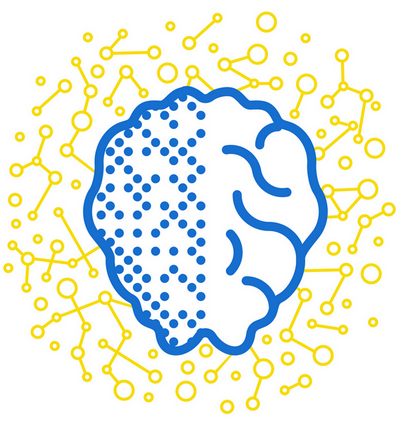
\includegraphics[height=1cm]{images/ipavlov-logo.png}}

\newcommand{\citepaper}[1]{\citetitle{#1} by \citeauthor{#1}}

%\graphicspath{{./images}}

%\usetheme{lucid}
\begin{document}


\begin{frame}
    \titlepage
\end{frame}


%\begin{frame}
%    \frametitle{Contents}
%    \tableofcontents
%\end{frame}


\section{Style Transfer not in Text}
\subsection{Image Style Transfer}


\begin{frame}    
\frametitle{Neural Style\footcite{NeuralStyle}}
\framesubtitle{Overview}
\begin{enumerate}
    \item Take three image:
    \begin{itemize}
        \item Image for content $\bm x_c$ (e.g., your grandma picture)
        \item Image for style $\bm x_s$ (e.g., ``La Muse'' by Picasso)
        \item Image of random noise $\bm x_r$, which we'll transform into the result
    \end{itemize}
    \item Pass them in VGG-19 and extract features
    \item Run optimization to make features of $\bm x_r$ to be close to $\bm x_c$ and be correlated like features of $\bm x_s$
\end{enumerate}

\begin{figure}
    \centering
    \begin{subfigure}[b]{0.3\textwidth}
        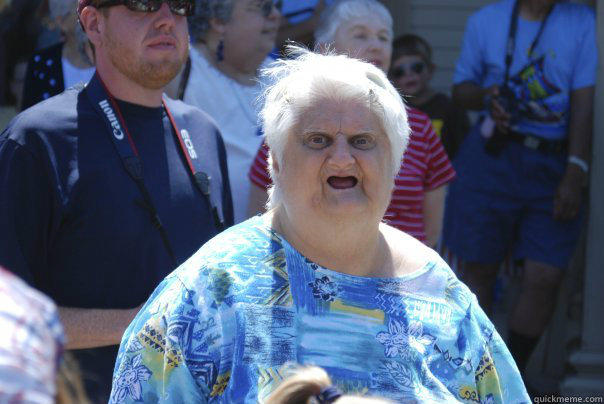
\includegraphics[width=\textwidth]{images/granny.jpg}
        \caption{Content $\bm x_c$}
    \end{subfigure}
    \begin{subfigure}[b]{0.3\textwidth}
        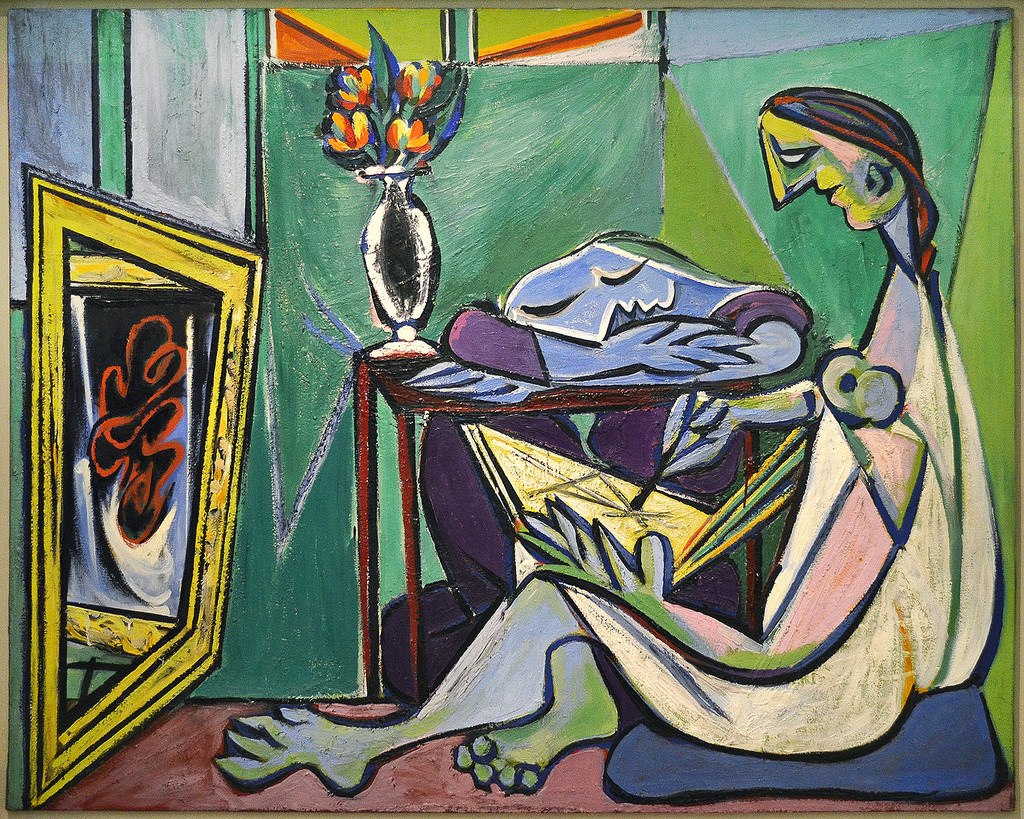
\includegraphics[width=\textwidth]{images/la-muse.jpg}
        \caption{Style $\bm x_s$}
        \vspace{-0.6cm}
    \end{subfigure}
    \begin{subfigure}[b]{0.3\textwidth}
        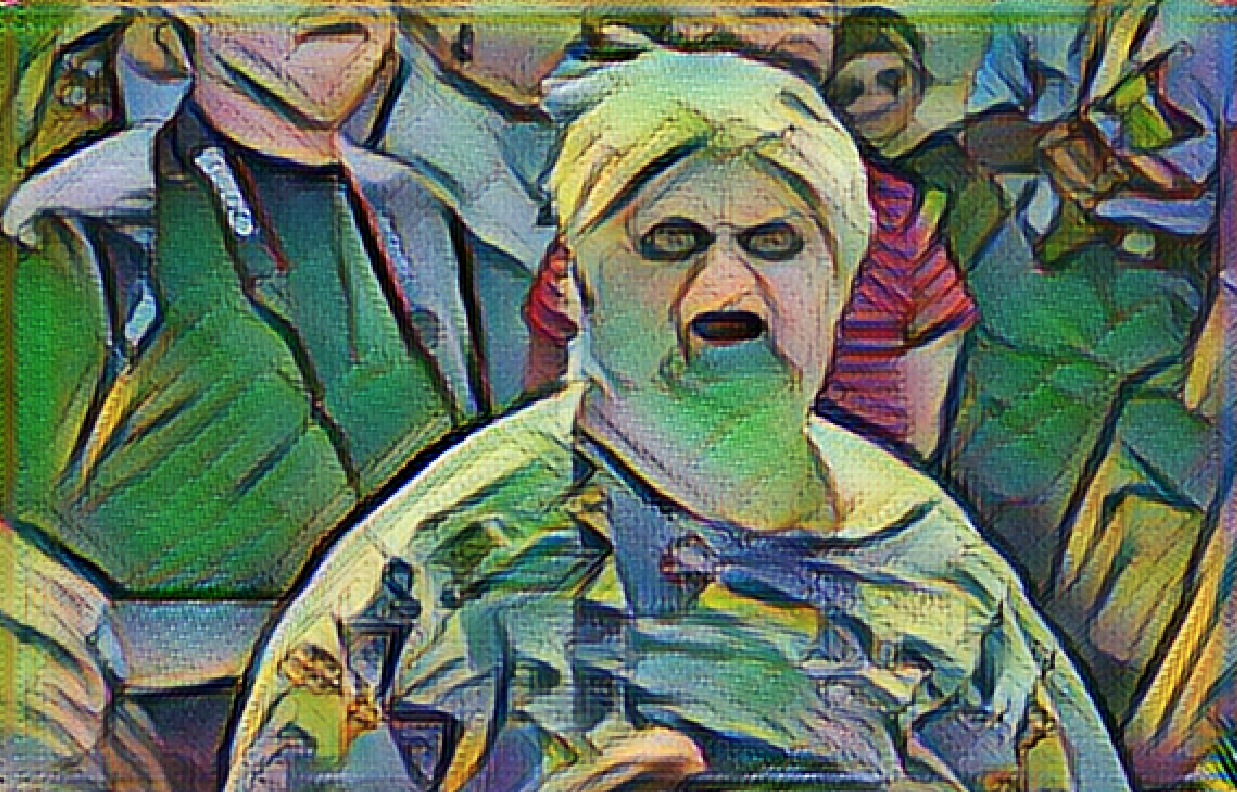
\includegraphics[width=\textwidth]{images/granny-muse-result}
        \caption{Result $\bm x_r$}
    \end{subfigure}
\end{figure}    
\end{frame}


\begin{frame}
\frametitle{Neural Style}
\framesubtitle{Computing loss}
To transfer style we should find such $\bm x_r$, which minimizes:

\[
\loss{\bm x_r} = \alpha \loss[\text{content}]{\bm x_r} + \beta \loss[\text{style}]{\bm x_r},
\]
where:
\begin{equation*}
\begin{split}
\loss[\text{content}]{\bm x_r} & = \frac{1}{2}\Vert F_c^k - F_r^k \Vert^2 \\
\loss[\text{style}]{\bm x_r} & = \frac{1}{k}\sum_{k} \frac{1}{4 n_k^2 m_k^2} \Vert F_s^k (F_s^k)^\top - F_r^k (F_r^k)^\top \Vert^2 \\
\end{split}
\end{equation*}

Here $F_c^k, F_s^k, F_r^k$ --- activations in $k$-th layer for $\bm x_c, \bm x_s, \bm x_r$; $n_k, m_k$ --- dimension and amount of features in $k$-th layer.
\begin{itemize}
    \item For $\loss[\text{content}]{\bm x_r}$ we use layer \#10.
    \item For $\loss[\text{style}]{\bm x_r}$ we use layers \#1, 3, 5, 9, 13!
\end{itemize}

\end{frame}


\begin{frame}
\frametitle{Neural style}
\framesubtitle{Extracting features}

To generate $F^k$, just pass $\bm x$ through VGG, obtain 3D matrix of activations (i.e. after ReLU was applied) and lay it out into 2D matrix:

\begin{figure}
    \centering
    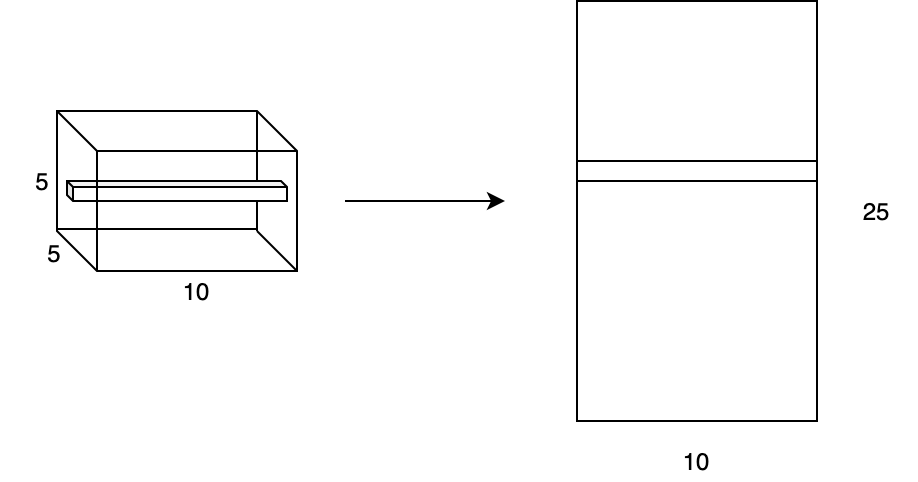
\includegraphics[width=0.8\textwidth]{images/neural-style-feature-extraction}
\end{figure}


\begin{itemize}
    \item $\loss[\text{content}]{\bm x_r}$ uses feature matrix $F^k$ as it is
    \item $\loss[\text{style}]{\bm x_r}$ uses $F^k \cdot (F^k)^\top$, i.e. a \textit{Gram matrix} of matrix $F^k$.
\end{itemize}

\end{frame}


\begin{frame}
\frametitle{Neural Style}
\framesubtitle{Gram matrix?}
Q. Why minimizing difference between Gram matrices transfers style?

A. It's equivalent to matching the distributions of features of $\bm x_r$ and $\bm x_s$.\footnote{\tiny{And why matching distributions transfers style? --- hren ego znaet}}
\bigbreak
Proof 1 (intuitive). Let $F = [f_1, ..., f_n]$, where $\bar{f} = 0$. Then Gram matrix $G = FF^\top$ is an empirical covariance (up to $\frac{1}{n-1}$):
\[
\hat{\text{Cov}}[f] = \frac{1}{n-1}\sum_{i=1}^n f_if_i^\top = \frac{1}{n-1}FF^\top
\]

\begin{itemize}
    \item Matching covariances of zero-mean distributions is like matching their first two moments
    \item Usually, matching first two moments is enough (e.g. for normal distribution they are sufficient statistics)
\end{itemize}

\end{frame}


\begin{frame}
\frametitle{Maximum Mean Discrepancy (MMD)\footcite{MMD}}
\framesubtitle{Gram matrix?}
Explanation 2 (strict). Let $F = [f_1, ..., f_n]$ and $D = [d_1, ..., d_m]$ (i.e. stack features as columns). Then minimizing $\Vert FF^\top - DD^\top \Vert^2$ is equivalent\footcite{DemystifyingNeuralStyle} to minimizing squared MMD between $f$ and $d$:

\begin{equation*}
\begin{split}
\text{MMD}^2[f, d] &= \frac{1}{n(n-1)} \sum_{i=1}^n \sum_{j\neq i}^n k(f_i, f_j) + \frac{1}{m(m-1)} \sum_{i=1}^m \sum_{j\neq i}^m k(d_i, d_j) \\
& \quad-\frac{2}{nm} \sum_{i=1}^n \sum_{j=1}^m k(f_i, d_j) \\
%\text{MMD}^2[f, d] & = \Vert \expect[f]{\phi(f)}  - \expect[d]{\phi(d)} \Vert^2 \\
%& = \expect[f_i, f_j]{\langle \phi(f_i), \phi(f_j) \rangle} - 2\expect[f_i, d_k]{\langle \phi(f_i), \phi(d_k) \rangle} + \expect[d_k, d_l]{\langle \phi(d_k), \phi(d_l) \rangle} \\
%& = \expect[f_i, f_j]{k(f_i, f_j)} - 2\expect[f_i, d_k]{k(f_i, d_k)} + \expect[d_k, d_l]{k(d_k, d_l)} \\
\end{split}
\end{equation*}

with polynomial kernel of the kind:
\[
k(f, d) = (f^\top d)^2
\]

Other kernels transfer style too (authors tried linear, polynomial and rbf).
\end{frame}


%\begin{frame}
%\frametitle{Differentiable Image Parametrizations\footcite{differentiable_image_parametrizations}}
%\framesubtitle{Making Neural Style work with non-VGG nets}
%
%
%
%\end{frame}


\begin{frame}
\frametitle{Adaptive Instance Normalization (AdaIN)\footcite{AdaIN_Style_Transfer}}
\framesubtitle{Any other ways to match feature distributions?}

Why another approach?
\begin{itemize}
    \item Style transfer via optimization procedure is slow
    \item But we can train a CNN autoencoder for each style!
    \item But then we'll be limited to these styles only
\end{itemize}

AdaIN to the rescue!
\begin{itemize}
    \item Pass $\bm x_c$ and $\bm x_s$ through VGG
    \item Extract activations $\bm f_c$ and $\bm f_s$ from layer \#11; compute their means and stds.
    \item Apply AdaIN for $\bm f_c$ by using statistics of $\bm f_s$:
\[
\hat{\bm f}_r = \text{AdaIN}(\bm f_c, \bm f_c) = \sigma(\bm f_s) \frac{\bm f_c - \mu(\bm f_c)}{\sigma(\bm f_c)} + \mu(\bm f_s)
\]
    \item Decode $\hat{\bm f}_r$ into $\bm x_r$ with CNN decoder
    \item Extract activations of $\bm x_r$ from VGG layers and compute losses
\end{itemize}

\end{frame}


\begin{frame}
\frametitle{Adaptive Instance Normalization (AdaIN)}
\framesubtitle{How to compute statistics and losses?}

Instance Normalization is like BatchNorm, but without batch dimension:
\[
\mu_{nc}(x) = \frac{1}{HW} \sum_{h, w} x_{nhwc} \qquad \sigma^2_{nc}(x) = \frac{1}{HW} \sum_{h,w} \left(x_{nhwc} - \mu_{nc}(x)\right)^2
\]

Loss function looks like:
\begin{equation*}
\begin{split}
\mathcal{L} & = \mathcal{L}_\text{content} + \gamma\sum_{k} \mathcal{L}_\text{style}^k \\
\mathcal{L}_\text{style}^k &= \Vert \mu(\bm f^k_r) - \mu(\bm f^k_s) \Vert + \Vert \sigma(\bm f^k_r) - \sigma(\bm f^k_s) \Vert \\
\mathcal{L}_\text{content} &= \Vert \bm f_r - \hat{\bm f}_r \Vert
\end{split}
\end{equation*}

\begin{figure}
\centering
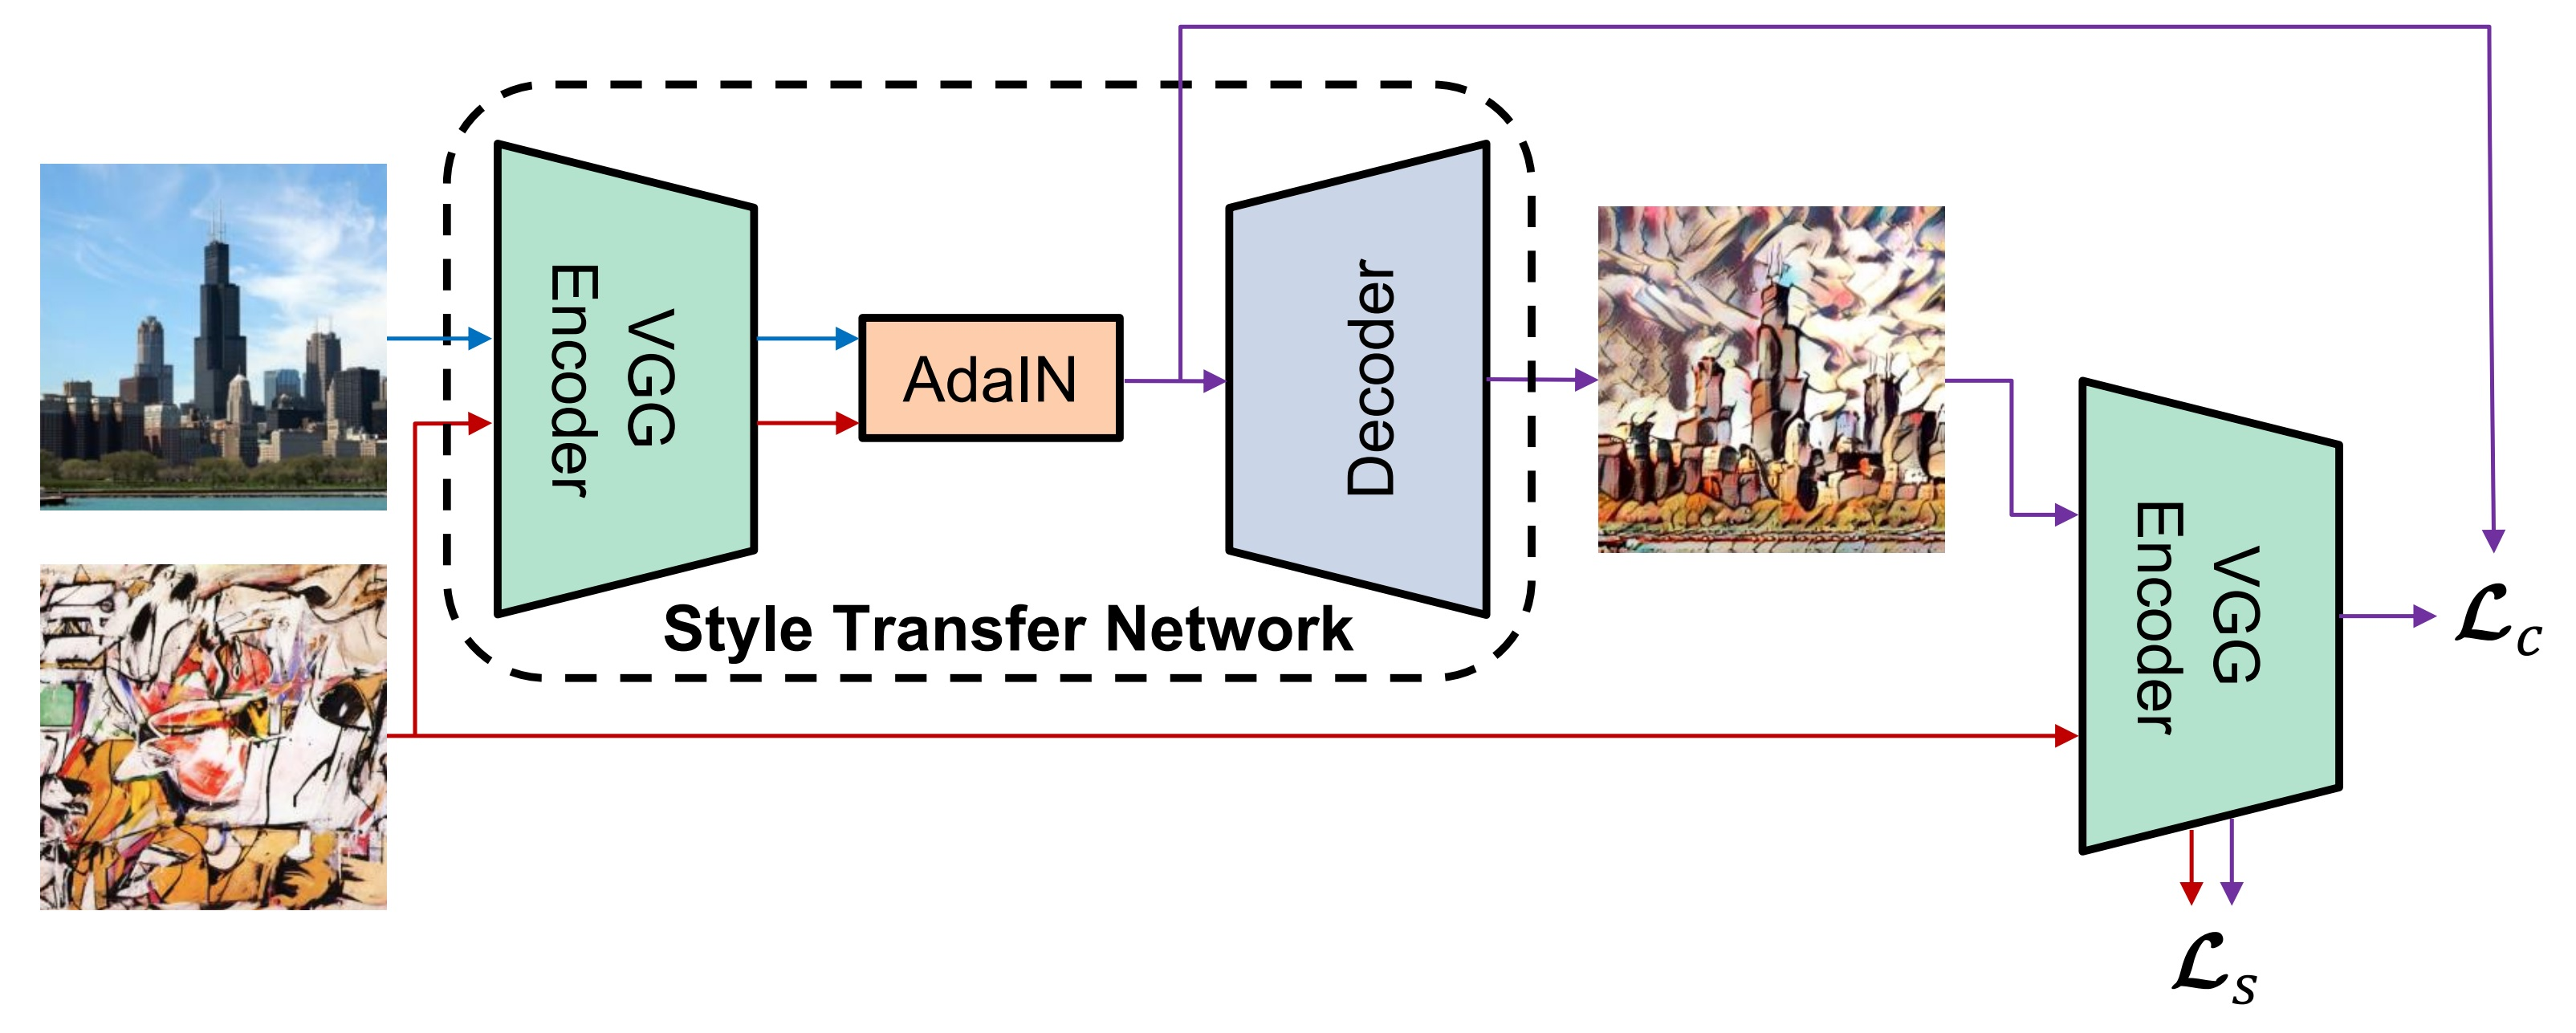
\includegraphics[width=0.7\textwidth]{images/AdaIN-style-transfer}
\end{figure}
\end{frame}


\begin{frame}
\frametitle{StyleGAN\footcite{StyleGAN}}
\framesubtitle{New GAN SotA!}

\begin{columns}
\begin{column}{6cm}

\begin{itemize}
    \item Based on ProGAN
    \item Uses two sources of input: latent code and noise
    \item Inputs are passed at every layer
    \item Uses AdaIN to transfer style
    \item Uses old CV tricks to make produced image look nicer
\end{itemize}

\end{column}
\begin{column}{6cm}

\begin{figure}
    \centering
    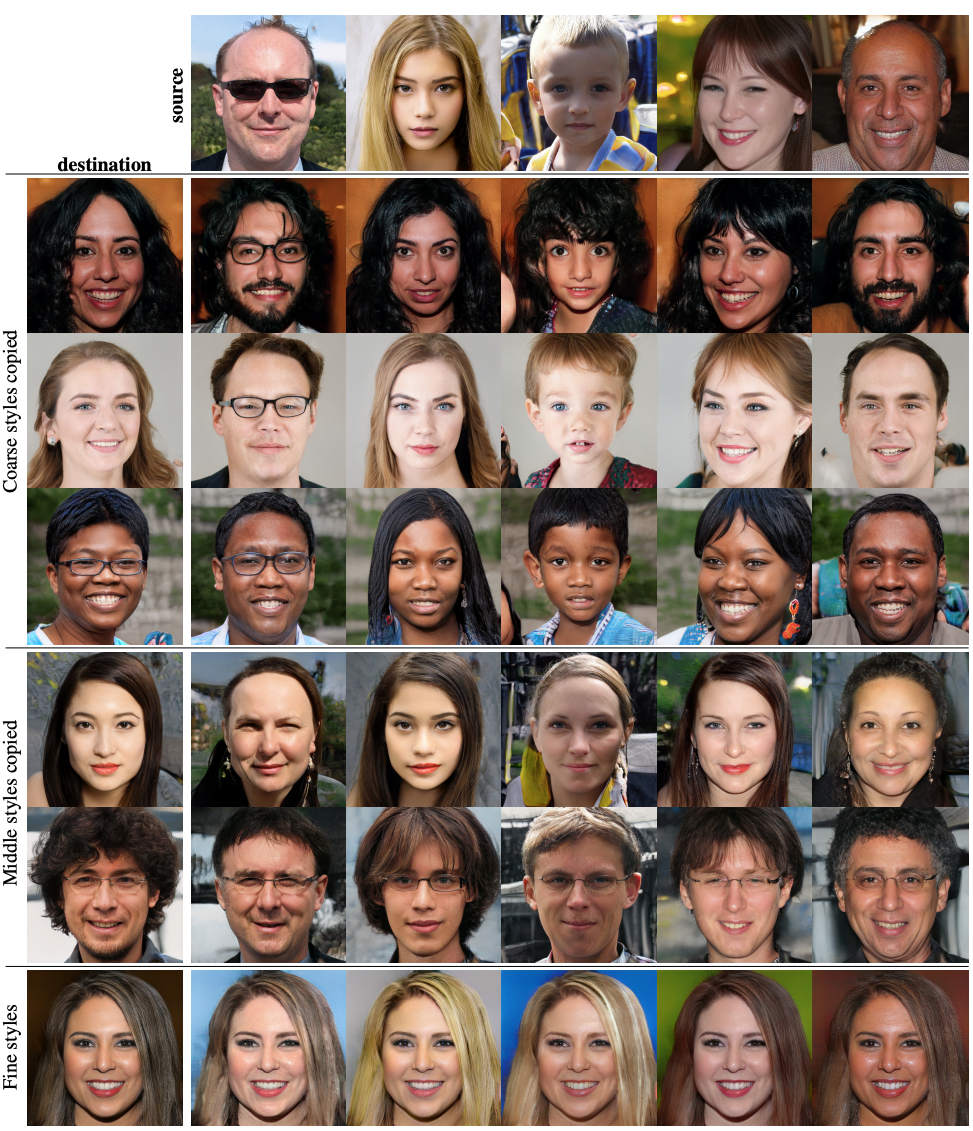
\includegraphics[width=0.8\textwidth]{images/style-gan-style-transfer}
\end{figure}

\end{column}
\end{columns}

\end{frame}


\begin{frame}
\frametitle{Style-based generator for GANs}
\framesubtitle{How it works}


\begin{columns}[T]

\begin{column}{6cm}
\begin{figure}
\centering
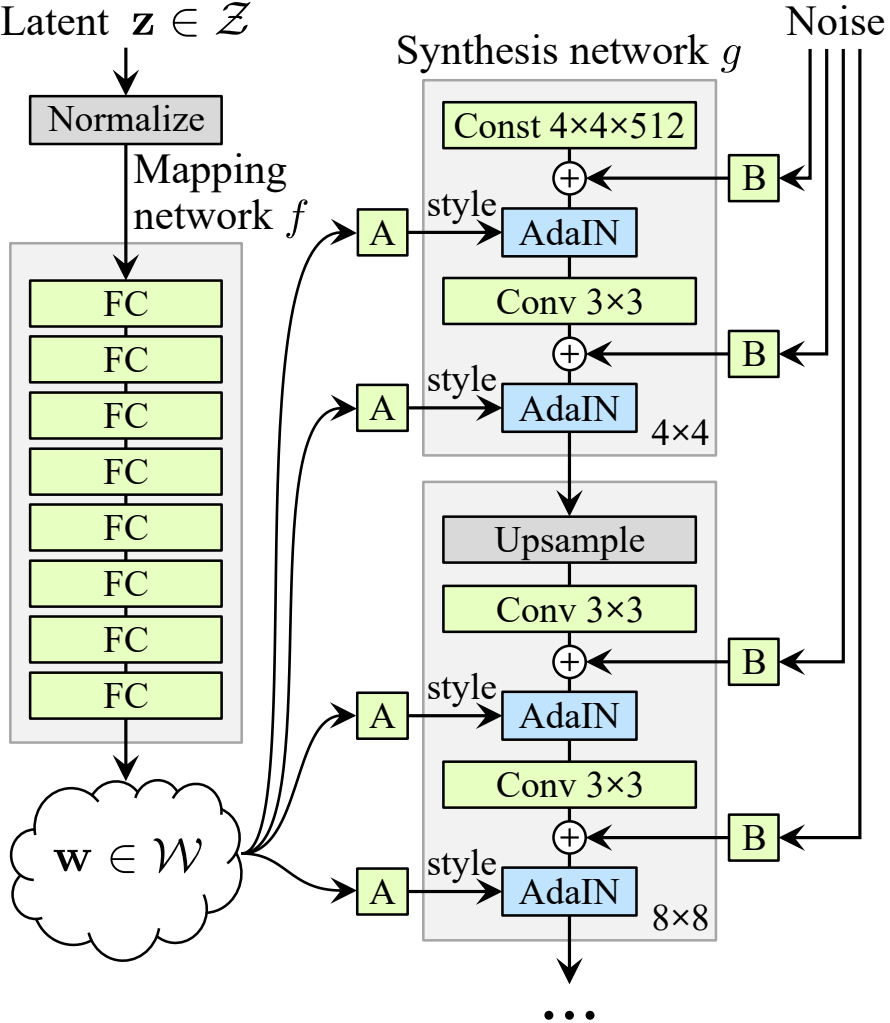
\includegraphics[width=\textwidth]{images/style-gan-architecture}
\end{figure}
\end{column}

\begin{column}{6cm}
\begin{enumerate}
    \item Embed latent code $z$ into $w$ via deep FFN (\textit{mapping network})
    \item Initialize Generator with constant input (which is learnt)
    \item Transform $w$ via affine mapping before passing to G
    \item Noise has size $H \times W \times 1$: it is broadcasted and scaled for each feature map
    \item New mean and std for AdaIN comes from $\bm y = A(w)$:
\[
\text{AdaIN}(\bm x, \bm y) = \bm y_\sigma \frac{\bm x - \mu(\bm x)}{\sigma (\bm x)} + \bm y_\mu
\]
\end{enumerate}
\end{column}
\end{columns}

\end{frame}


\begin{frame}
\frametitle{StyleGAN}
\framesubtitle{Some (not strict) architectural implications and other interesting things}

\begin{columns}[T]
\begin{column}{5cm}
\begin{itemize}
\item Passing noise at every layer allows styles to localize in the network
\end{itemize}

\begin{figure}
    \centering
    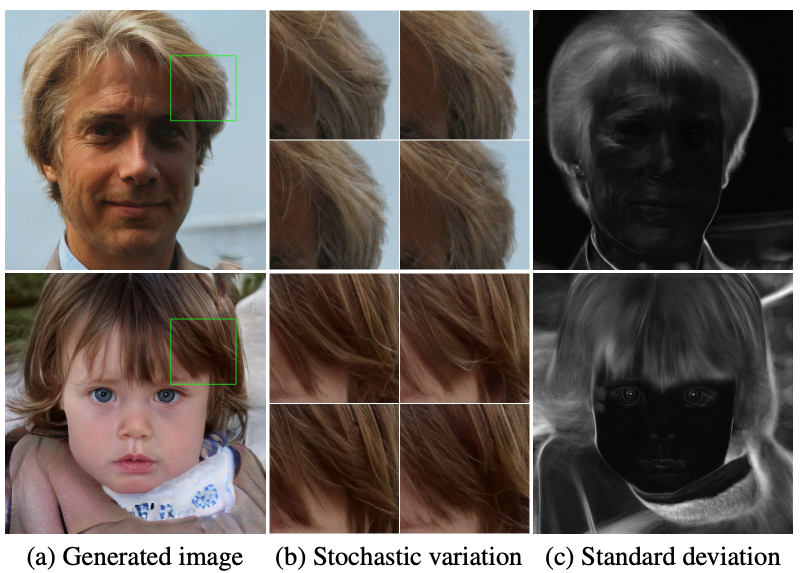
\includegraphics[width=\textwidth]{images/stylegan-local-styles}
\end{figure}
\end{column}

\begin{column}{7cm}
\begin{itemize}
    \item Mapping Network eases disentanglement:
    \begin{itemize}
        \item If $z \sim \mathcal{N}(0,1)$ is disentangled, then mapping $z \mapsto features$ is warped, because $G$ should remove unexisting combinations of features
        \item Mapping Network takes this part, freeing generator's capacity
    \end{itemize}
    \item Passing latents and noise at every layer allows generator not to carry all the information through the whole forward pass
\end{itemize}
\end{column}
\end{columns}

\begin{itemize}
    \item They used non-saturating loss with $R_1$ regularization for FFHQ!
\[
\expect[z]{\log D_\theta(G_\phi(z))} \to \max_\phi \qquad\qquad R_1(\theta) = \frac{\gamma}{2}\expect[p_{data}]{\Vert D_\theta (x) \Vert^2}
\]
\end{itemize}

\end{frame}


\begin{frame}
\frametitle{StyleGAN}
\framesubtitle{Scores}
FID (Frechet Inception Distance) is calcluated like:
\begin{itemize}
    \item Generate a mini-dataset from generator (5k-50k samples)
    \item Pass real and generated data through Inception-v3
    \item Calculate empirical means and covariances of activations in some middle layer
    \item Calculate FID as:
\[
\text{FID} = \Vert\mu_r - \mu_g\Vert^2 + \text{tr} (\Sigma_r + \Sigma_g - 2 (\Sigma_r \Sigma_g)^{1/2}),
\]
\end{itemize}

Something like ablation study:
\begin{figure}
\centering
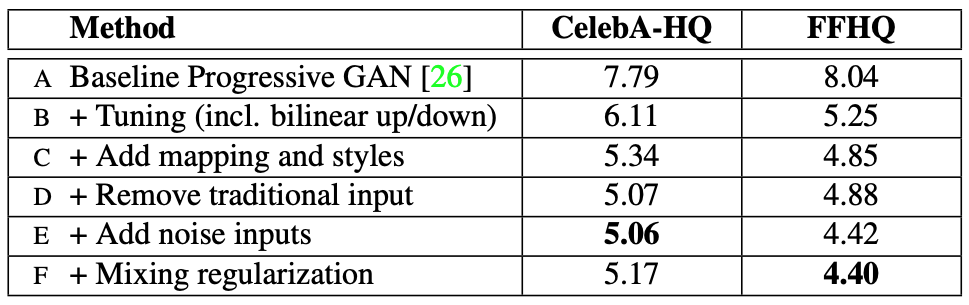
\includegraphics[width=0.8\textwidth]{images/stylegan-scores}
\end{figure}

\end{frame}



\begin{frame}
\frametitle{CycleGAN\footcite{CycleGAN}}
\framesubtitle{Overview}
We have a dataset of zebras and a dataset of horses (unparallel!), and want to transform zerbras to horses and horses to zebras
\begin{itemize}
    \item Train two GANs: a GAN per each dataset
    \item Feed images of opposite domain to generators (instead of noise)
    \item Add \textit{cycle consistency} loss
%: transformation $horse \xrightarrow{G_\text{zebra}} zebra \xrightarrow{G_\text{horse}} horse$ should return the same $horse$!
\end{itemize}


\begin{columns}[T] % contents are top vertically aligned
\begin{column}[T]{5cm}
\begin{figure}
    \vspace{1cm}
    \centering
    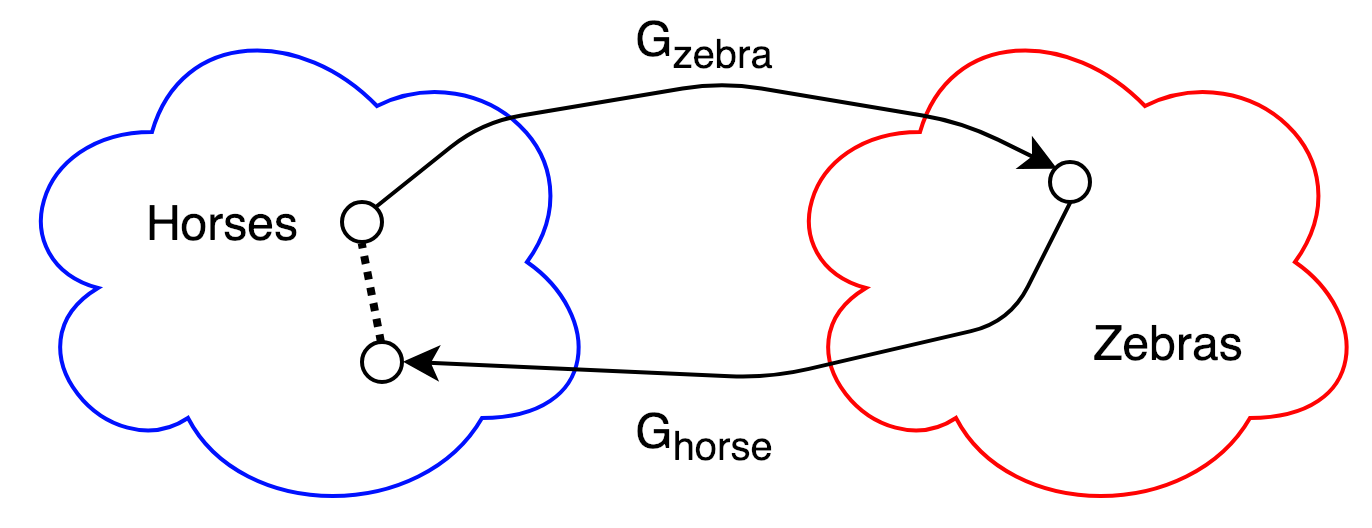
\includegraphics[width=\textwidth]{images/cycle-gan-cycle-consistency}
    \caption{Cycle consistency}
\end{figure}
\end{column}
\begin{column}[T]{5cm}
\begin{figure}
    \centering
    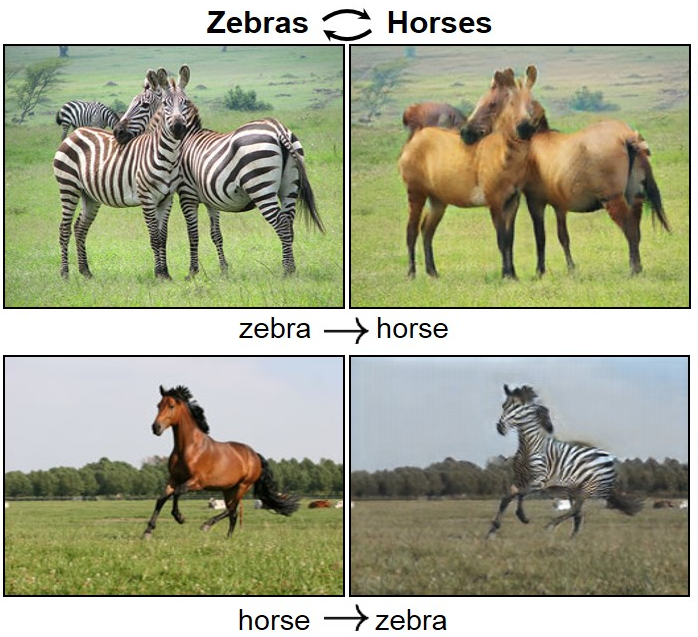
\includegraphics[width=0.8\textwidth]{images/cycle-gan-horses}
    \caption{Samples from CycleGAN, trained on horses and zebras}
\end{figure}
\end{column}
\end{columns}
\end{frame}


\begin{frame}
\frametitle{CycleGAN}
\framesubtitle{How to compute losses}
\begin{equation*}
\begin{split}
\mathcal{L} &= \mathcal{L}_\text{Zebra GAN} + \mathcal{L}_\text{Horse GAN} + \alpha\mathcal{L}_\text{cycle} \\ 
\mathcal{L}_\text{Zebra GAN} &= \expect[z \sim p_z]{\log \textcolor{red}{D_z}(\textcolor{red}{z})} + \expect[h \sim p_h]{\log(1 - \textcolor{red}{D_z}(\textcolor{red}{G_z}(\textcolor{blue}{h})))} \\
\mathcal{L}_\text{Horse GAN} &= \expect[h \sim p_h]{\log \textcolor{blue}{D_h}(\textcolor{blue}{h})} + \expect[h \sim p_h]{\log(1 - \textcolor{blue}{D_h}(\textcolor{blue}{G_h}(\textcolor{red}{z})))} \\
\mathcal{L}_\text{cycle} &= \expect[z \sim p_z]{\Vert \textcolor{red}{G_z}(\textcolor{blue}{G_h}(\textcolor{red}{z})) - \textcolor{red}{z} \Vert_1} + \expect[h \sim p_h]{\Vert \textcolor{blue}{G_h}(\textcolor{red}{G_z}(\textcolor{blue}{h})) - \textcolor{blue}{h} \Vert_1} \\
\end{split}
\end{equation*}


\begin{figure}
    \centering
    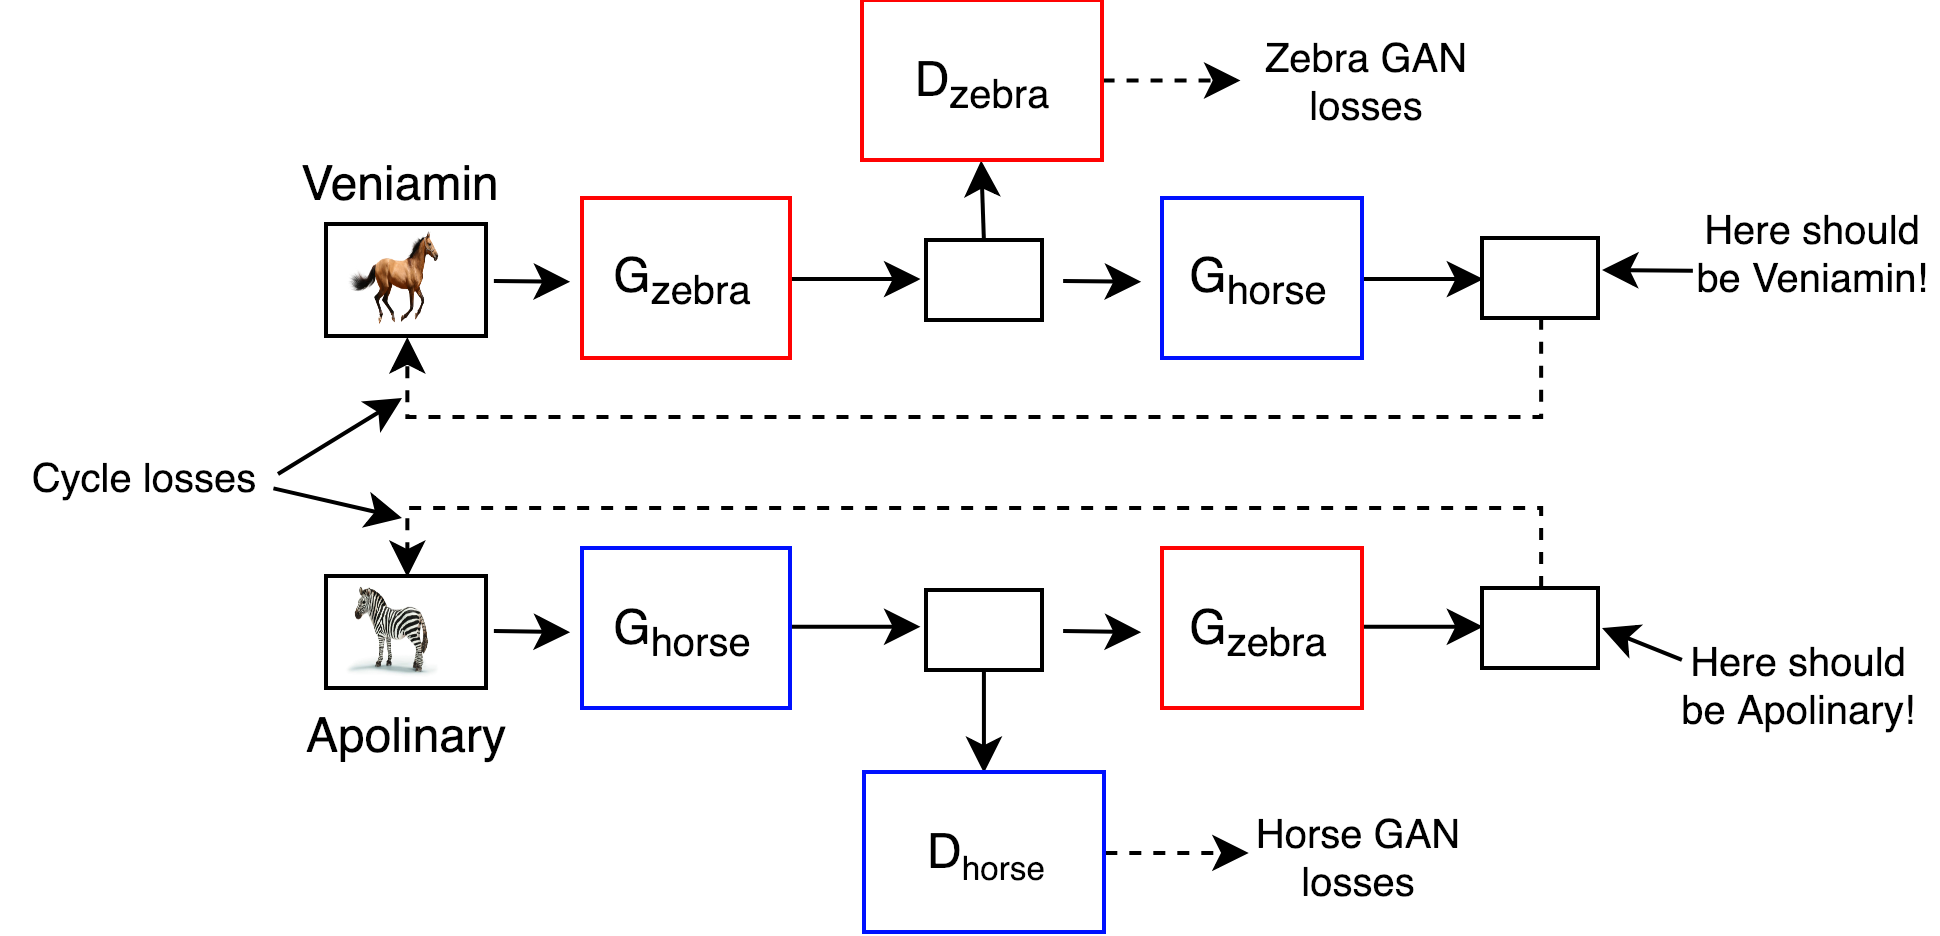
\includegraphics[width=0.8\textwidth]{images/cycle-gan.png}
\end{figure}

\end{frame}


%\subsection{Voice Style Transfer (a tiny bit)}
%
%
%\begin{frame}
%    \frametitle{Voice Style Transfer}
%    \framesubtitle{An Example of Lists}
%    \begin{itemize}
%        \item 1
%        \item 2
%        \item 3
%    \end{itemize}
%\end{frame}
%

\section{Style Transfer in Text}
%\subsection{(V $\mid$ A $\mid$ W $\mid$ AR)AE}


\begin{frame}
\frametitle{Unsupervised Neural Machine Translation\footcite{UnsupervisedMT}\footcite{PhraseBasedUNMT}}
How to do unsupervised NMT in 2k18:
\begin{itemize}
    \item Learn to translate in both directions
    \item Use shared encoder, initialized with cross-aligned word embeddings
    \item Use shared decoder, which recieves language-dependent BOS token
    \item Pretrain model with denoising autoencoding (words are dropped and swapped)
    \item Use back-translation (a lot)!
    \item And do not forget about fastText BPE (+3 BLEU)
    \item Switch to phrase-based statistical MT, because it works better (for  $\sim$ 3 BLEU)
\end{itemize}

\end{frame}


%\begin{frame}
%\frametitle{Unsupervised Word Translation\footcite{UnsupervisedWT}}
%\framesubtitle{Cross-aligning word embeddings}
%
%\begin{itemize}
%    \item Take two monolingual corpora
%    \item 
%\end{itemize}
%
%\end{frame}


\begin{frame}
\frametitle{First works on Style Transfer \footcite{TowardControlledGenerationOfText}}

\begin{itemize}
    \item Train VAE on text
    \item Concatenate sentiment flag $c$ to $z$
    \item Penalize decoder for bad classifications of decoded sentences
    \item Some other training details:
    \begin{itemize}
        \item Pretrain classifier on normal dataset
        \item Minimize entropy of classifier as additional loss
        \item Encode decoded sentence and penalize decoder if original $z$ has low probability
        \item Soft embeddings from decoder are passed to classifier
    \end{itemize} 
\end{itemize}

\begin{figure}
\centering
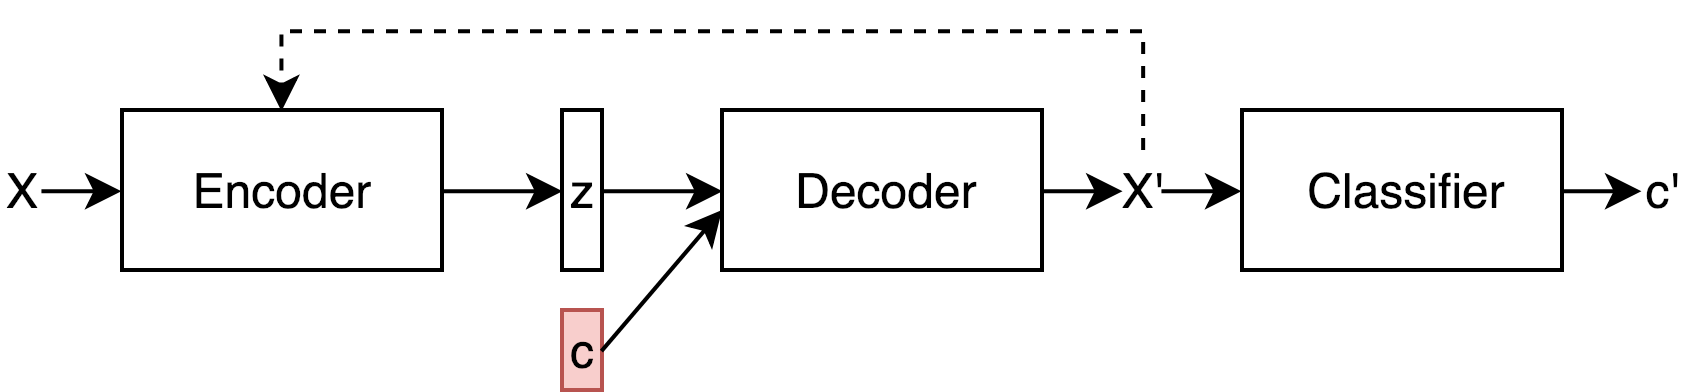
\includegraphics[width=0.8\textwidth]{images/controlled-generation}
\end{figure}
\end{frame}


\begin{frame}
\frametitle{Style Transfer via Professor-Forcing\footcite{StyleTransferByCrossAlignment}}
\begin{itemize}
    \item Both encoder and decoder are shared and trained to autoencode
    \item Both encoder and decoder receive sentiment flag $\bm y_c$
    \item Train 2 discriminators $D_1$ and $D_2$ for each domain (positive and negative sentiment)
    \item Discriminators receive hidden states instead of word embeddings (i.e. Professor-Forcing)
\end{itemize}

\begin{figure}
\centering
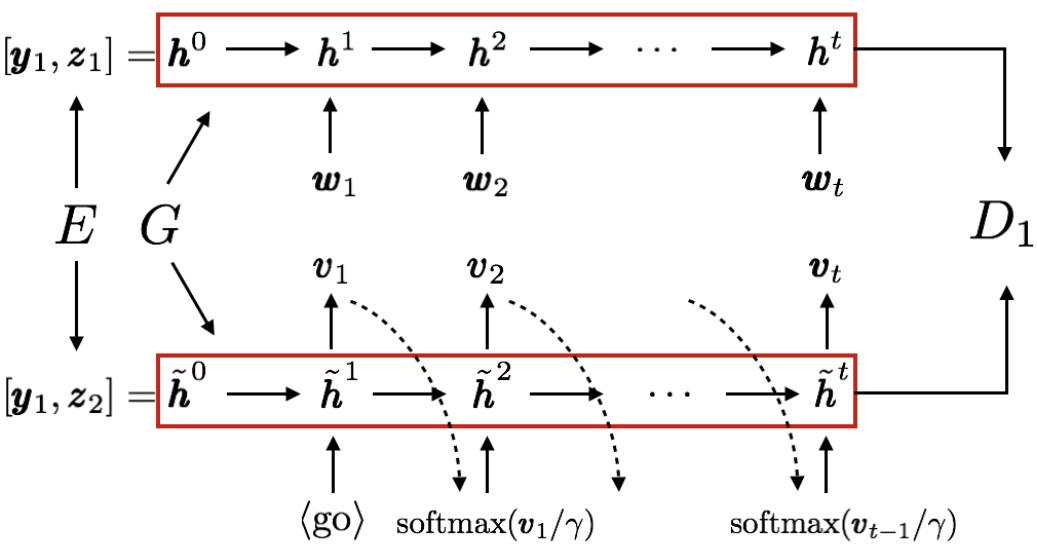
\includegraphics[width=0.7\textwidth]{images/style-transfer-via-professor-forcing}
\end{figure}
\end{frame}


\begin{frame}
\frametitle{How to measure style transfer?\footcite{Text_Style_Transfer_Exploration_and_Evaluation}}

\begin{itemize}
    \item \textit{Content preservation}:
    \begin{enumerate}
        \item Embed words of transfered and original sentence via GloVe
        \item Transform into a single vector from avg/min/max pooling
        \item Compute cosine distance with original sentence
    \end{enumerate}
    \item \textit{Transfer strength}: train classifier and measure its accuracy
    \item BLEU (or any other MT metric)
    \item Human Evaluations
\end{itemize}

\end{frame}



\begin{frame}
\frametitle{What if care about sentiment transfer only?\footcite{SentimentTransferWithRL}}
\framesubtitle{Let's train the model just to replace positive words with negative}
\begin{columns}
\begin{column}{6cm}
\begin{itemize}
    \item Train two networks: neutralization net $N$ and emotionalization net $E$
    \item $N$ is LSTM net, which detects and removes emotional words
    \item $E$ is encoder with two decoders, which receives neutralized sentence and inserts emotional words
    \item Pretrain $N$ on classification, $E$ on autoencoding
    \item After pretraining, we can train with policy gradients
\end{itemize}
\end{column}

\begin{column}{6cm}
\begin{figure}
\centering
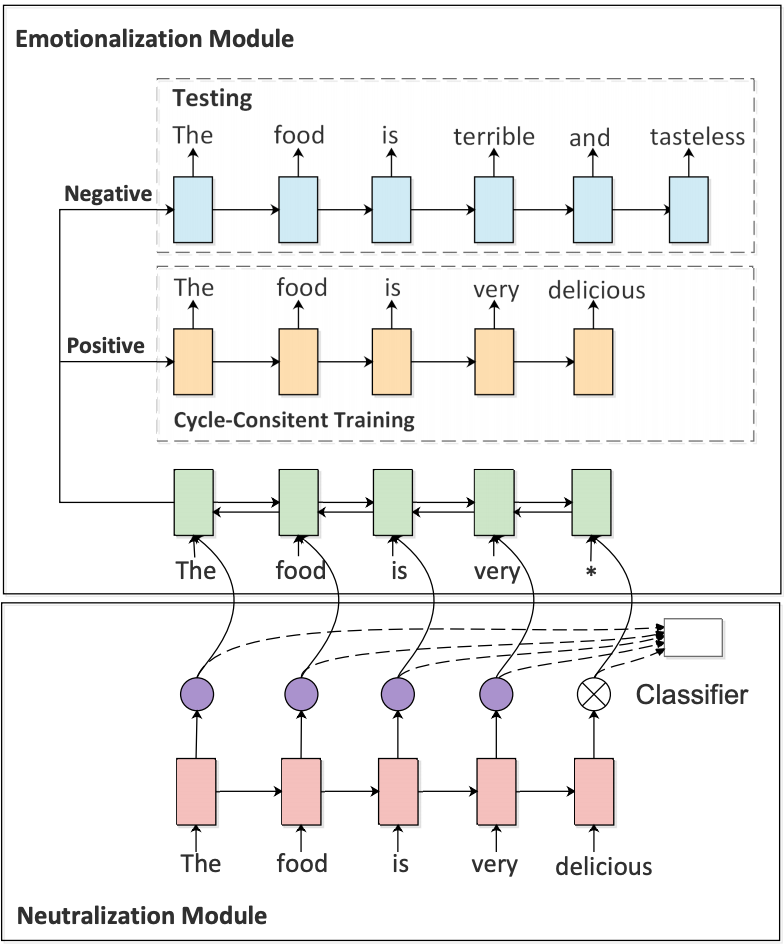
\includegraphics[width=0.8\textwidth]{images/rl-sentiment-transfer}
\end{figure}
\end{column}
\end{columns}

\end{frame}


\begin{frame}
\frametitle{What if care about sentiment transfer only?}
\framesubtitle{Some details}
\begin{itemize}
    \item How to pretrain neutralization module $N$:
    \begin{itemize}
        \item Let $h_i$ is the $i$-th output of $N$ and we have $T$ words
        \item Compute attention weights $\alpha_i$ of $h_i$ with $h_T$
        \item Predict sentiment class as $y = \sigma(Wc)$ where $c = \sum_i \alpha_i h_i$
        \item Discretize $\alpha_i$ and generate synthetic training dataset for $N$
    \end{itemize}
    \item How to rl:
    \begin{itemize}
        \item $E$ is trained without RL, just train him to reconstruct neutralized sentence (``cycle approach''?)
        \item Train module $N$ with policy gradient:
\end{itemize}
\end{itemize}
\begin{equation*}
\begin{split}
\nabla_\theta J & = \expect{R \cdot \nabla_\theta \log P_N(\hat{\alpha} | x)} \\
\text{with reward: } R & = (1 + \beta^2) \cdot \frac{\text{BLEU} \cdot \text{Confidence}}{\beta^2 \cdot \text{BLEU} + \text{Confidence}}
\end{split}
\end{equation*}
\end{frame}


\begin{frame}
\frametitle{Style Transfer via Machine Translation\footcite{StyleTransferViaBackTranslation}}
\begin{itemize}
    \item Train EN$\to$FR and FR$\to$EN NMT models
    \item Translate with EN$\to$FR, encode with FR$\to$EN model
    \item Train to style decoders for each style
    \item Train classifier to ``fine-tune'' decoders
    \item Datasets used: male$\leftrightarrow$female Yelp reviews and democratic$\leftrightarrow$republican facebook posts
\end{itemize}

\begin{figure}
\centering
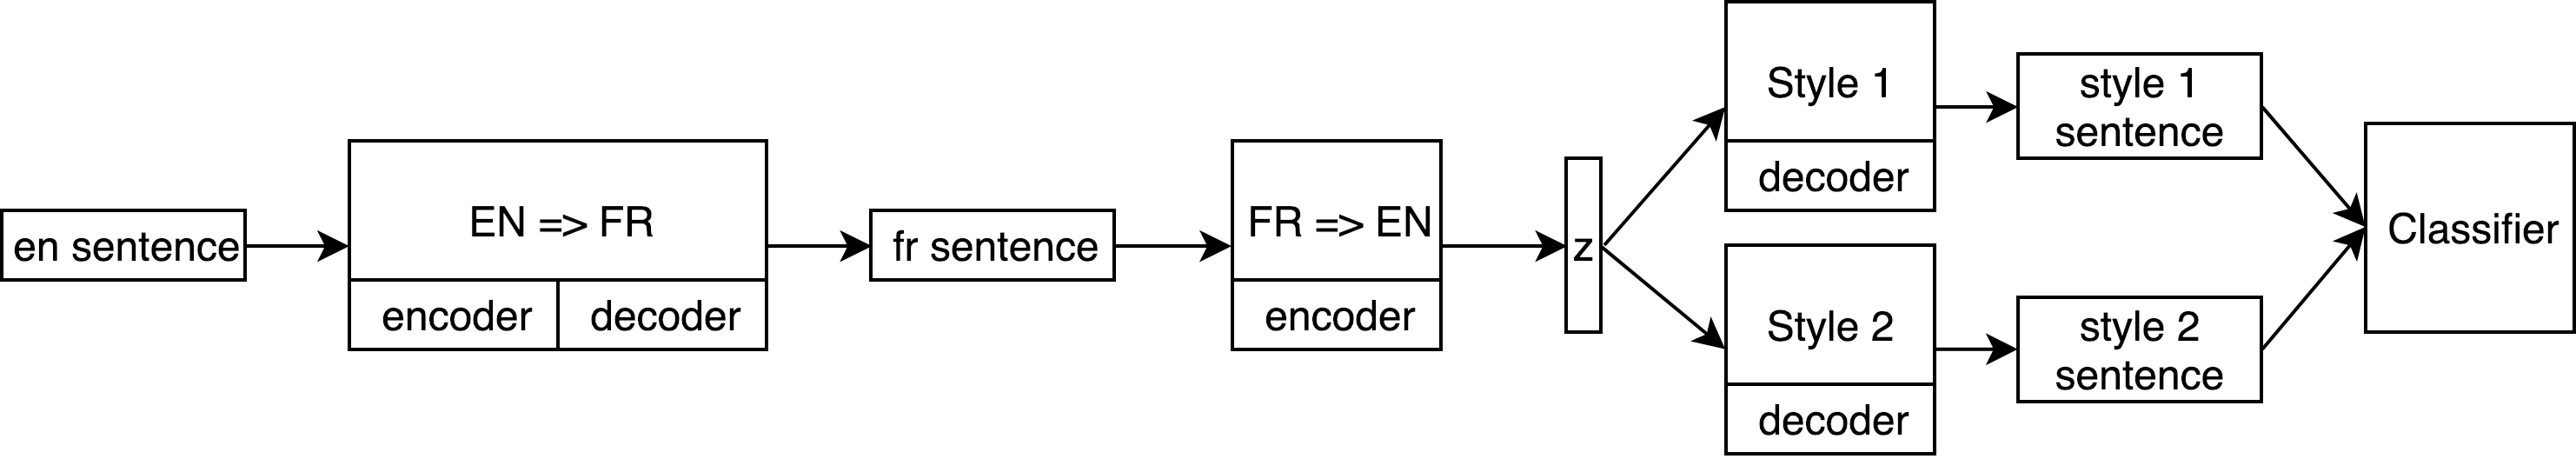
\includegraphics[width=\textwidth]{images/style-transfer-via-mt.png}
\end{figure}
\end{frame}


\begin{frame}
\frametitle{Style Transfer via Machine Translation}
\framesubtitle{Some samples}

Some samples of male$\leftrightarrow$female transfers
\begin{table}[]
\small
\begin{tabular}{p{5cm}|p{5cm}}
Input & Result \\
\hline
(M) \makecell[l]{my wife ordered country \\ fried steak and eggs} & (F) \makecell[l]{my husband ordered the chicken steak \\ and eggs. salad and the fries} \\
(M) \makecell[l]{the place is small but \\ cosy and very clean} & \makecell[l]{(F) the place is great but \\ very clean and very friendly} \\
(F) save yourself the huge headaches  & (M) you are going to be disappointed  \\
(F) \makecell[l]{my husband ordered the salad \\ and the dressing - lrb - blue \\ cheese - rrb - was watered down} & \makecell[l]{(M) my wife ordered the mac-ncheese \\ and the salad - lrb - \$ \\ 00 minutes - rrb - was cooked}
\end{tabular}
\end{table}

\end{frame}


\begin{frame}
\frametitle{Style Transfer with LM discriminators\footcite{StyleTransferWithLMDiscriminators}}
\framesubtitle{Overview}
\begin{itemize}
    \item Train encoder-decoder architecture as usual
    \item Train LM for each domain
    \item Let $x, y$ be positive and negative sentences. Then decoder $G_y$ is trained to spoof $\text{LM}_x$
\end{itemize}

\begin{figure}
\centering
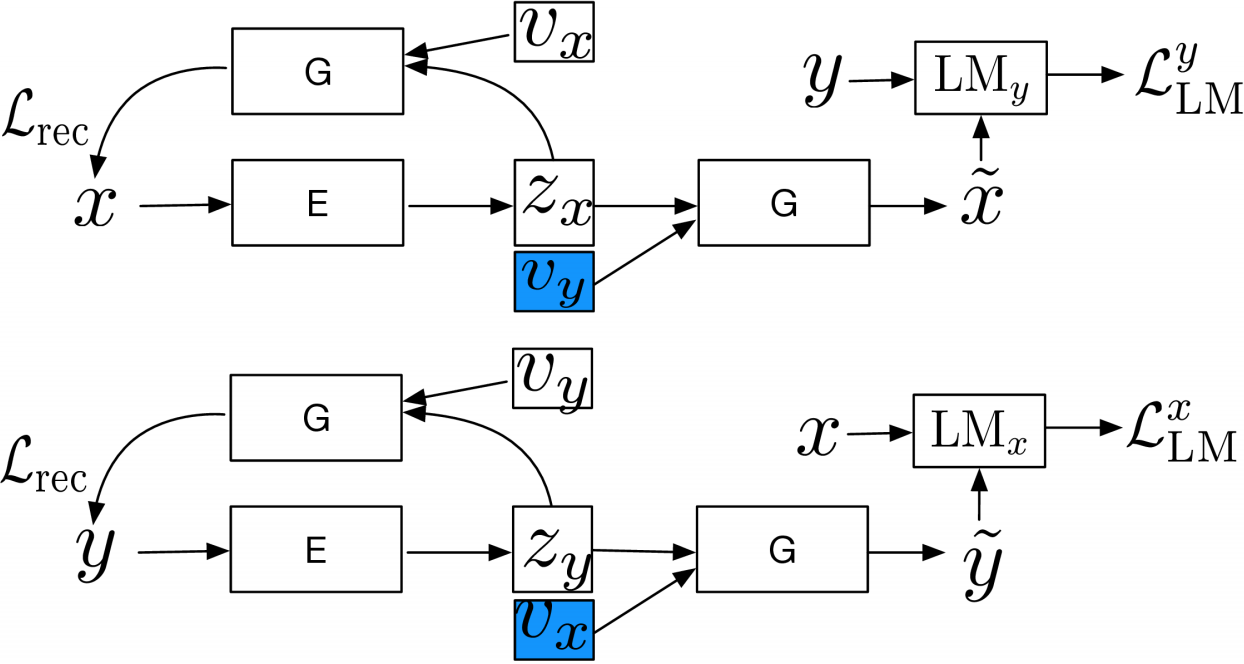
\includegraphics[width=0.7\textwidth]{images/style-transfer-via-lm-discriminators-architecture}
\end{figure}
\end{frame}

\begin{frame}
\frametitle{Style Transfer with LM discriminators}
\framesubtitle{How we compute losses}
\begin{itemize}
\item Normal autoencoding CE loss for encoder-decoder
\item Loss to train LM (here $\tilde{y}$ is transfered sentence):
\[
\loss{\text{LM}_x} = -\expect{\log p_{\text{LM}_x}(x)} + \gamma \expect{\log p_{\text{LM}_x}(\tilde{y})}
\]
\end{itemize}
\begin{itemize}
\item Adversarial loss to train decoder
\end{itemize}
\[
\mathcal{L}_{adv}(G_y) \approx \expect{\sum_{t=1}^T \langle \tilde{p}_t, \log \hat{p}_t \rangle} \text{ where } \tilde{p}_t, \hat{p}_t \text{ are } G_y \text{ and } \text{LM}_x \text{ probabilities}
\]

\begin{columns}
\begin{column}{6cm}
\begin{figure}
\centering
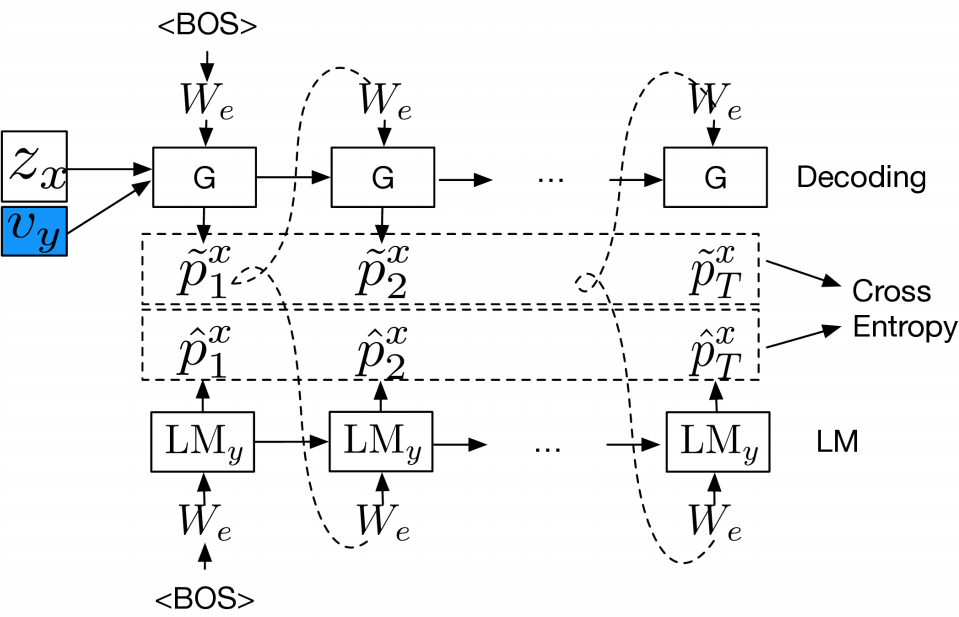
\includegraphics[width=\textwidth]{images/style-transfer-with-lm-discriminators-soft-embed}
\end{figure}    
\end{column}

\begin{column}{6cm}
\begin{itemize}
    \item Decoded sentence is passed to LM as soft Gumbel
    \item Additional tricks: normalize LM loss by length (LM prefers short sentences) and make $\tilde{x}$ to have the same length as $x$ 
\end{itemize}
\end{column}
\end{columns}
\end{frame}


\begin{frame}
\frametitle{Back-translation strikes again\footcite{StyleTransferViaSoftBackTranslation}}
\begin{itemize}
    \item Usual encoder-decoder architecture, but now we have \textit{sentence attributes} instead of style flags
    \item Train as a general auto-encoder
    \item Train with general back-translation:
    \begin{enumerate}
        \item Transfer $x$ with attributes $l$ into $y$ with attributes $l'$
        \item Transfer $y$ with attributes $l'$ into $x$ with attributes $l$ again
    \end{enumerate}
    \item Add \textit{interpolated reconstruction}:
    \begin{enumerate}
        \item Transfer $x$ with attributes $l$ into $y$ with attributes $l'$
        \item Encode $x$ into $z_x$ and encode $y$ into $z_y$
        \item Generate $z_{xy}$: with some probability $p_i$ replace $i$-th coordinate in $z_y$ with value from $z_x$
        \item Decode $z_{xy}$ into $\hat{x}$ with labels $l$
    \end{enumerate}
\end{itemize}
\begin{figure}
\centering
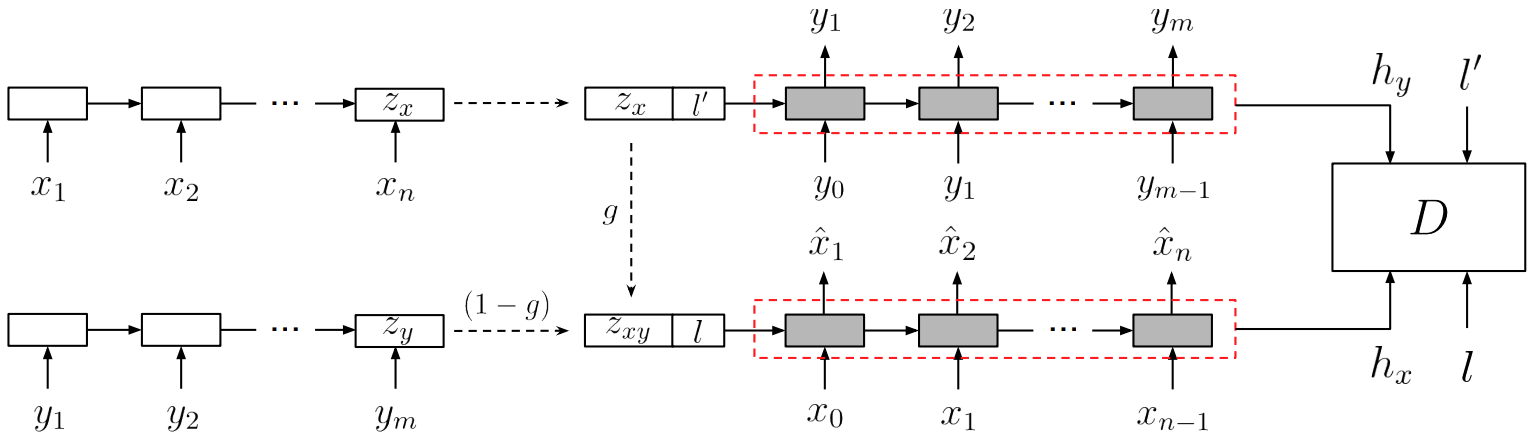
\includegraphics[width=0.8\textwidth]{images/interpolated-bt-architecture}
\end{figure}

\end{frame}


\begin{frame}
\frametitle{Back-translation strikes again}
\framesubtitle{Adversarial loss details}

Let's also add discriminator loss:
\begin{itemize}
    \item Discriminator $D$ recieves hidden states from decoder and sentence attributes
    \item Adversarial loss includes three kind of pairs:
    \begin{itemize}
        \item Auto-encoded sentence $x$, real attributes (as true sample)
        \item Auto-encoded sentence $x$, mistmatched attributes (as fake sample)
        \item Transfered sentence $y$, ``real'' attributes (as fake sample)
    \end{itemize}
    \item Given attributes $l'$, adversarial loss is:
\[
\mathcal{L}_\text{adv} = \expect{2\log D(h_x, l) + \log (1 - D(h_y, l')) + \log(1 - D(h_x, l'))}
\]
(expectation is taken over $(x,l) \sim p_\text{data}, y \sim p_G(\cdot|z_x, l')$)
\end{itemize}
\end{frame}


\begin{frame}
\frametitle{Back-translation strikes again}
Some samples from old$\leftrightarrow$new Shakespeare:
\begin{figure}
\centering
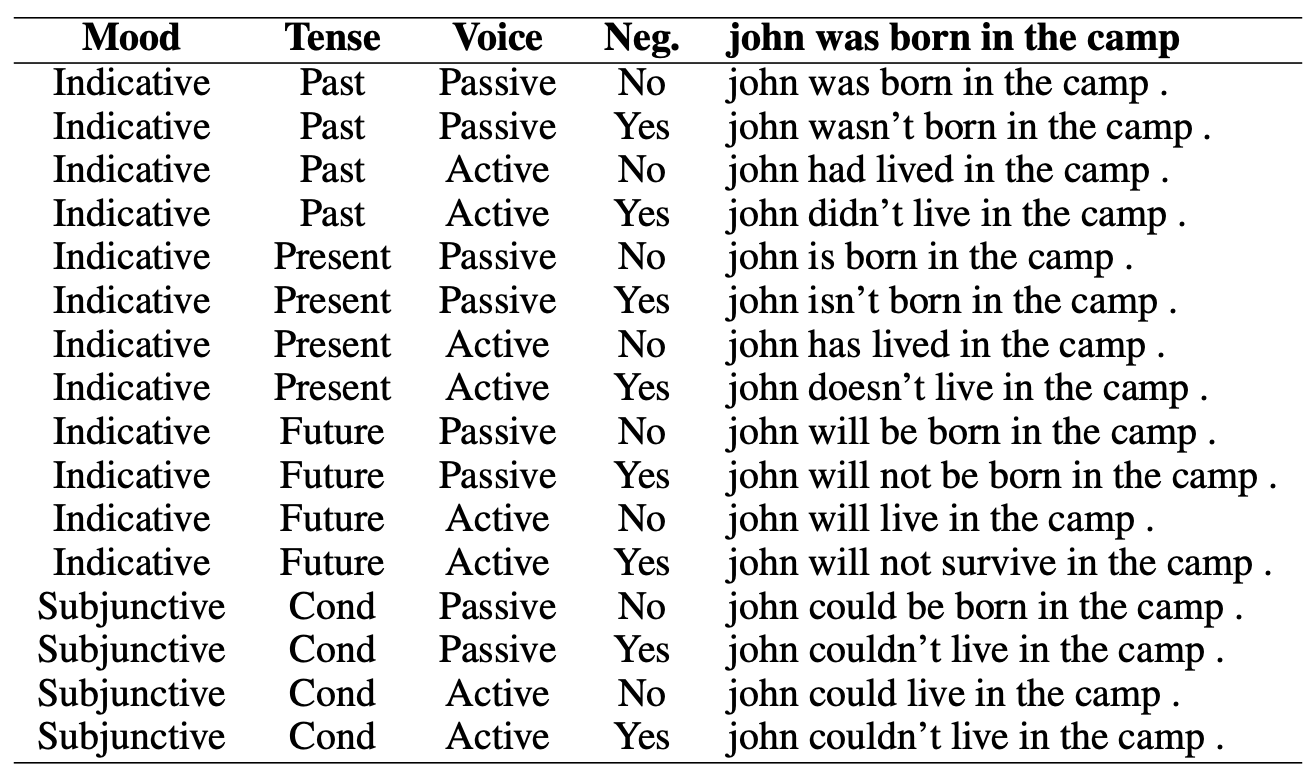
\includegraphics[width=0.6\textwidth]{images/interpolated-bt-samples}
\end{figure}
\end{frame}


\begin{frame}
\frametitle{Style Transfer without disentagled things\footcite{MultipleAttributeTextStyleTransfer}}
\framesubtitle{Or a little bit more of back-translation}
\begin{itemize}
    \item Train usual Unsupervised NMT system (back-translation is crucial)
    \item Do not use discriminator to remove style information from encodings, because it does not work anyway: if one trains a classifier after training is done, then it will still be able to guess the style attributes in content vector with 90\% accuracy
    \item Pass attribute embedding as BOS token to decoder
    \item Add attention to decoder on max-pooled parts of encoder states: run non-overlapping window of size $5$ over encoder hidden states and max-pool everything inside a window
    \item Also learn biases in decoder output softmax for each attribute characteristic (and average them later)
\end{itemize}
\end{frame}


\begin{frame}
\frametitle{Style Transfer without disentagled things}
Samples from the model:
\begin{figure}
\centering
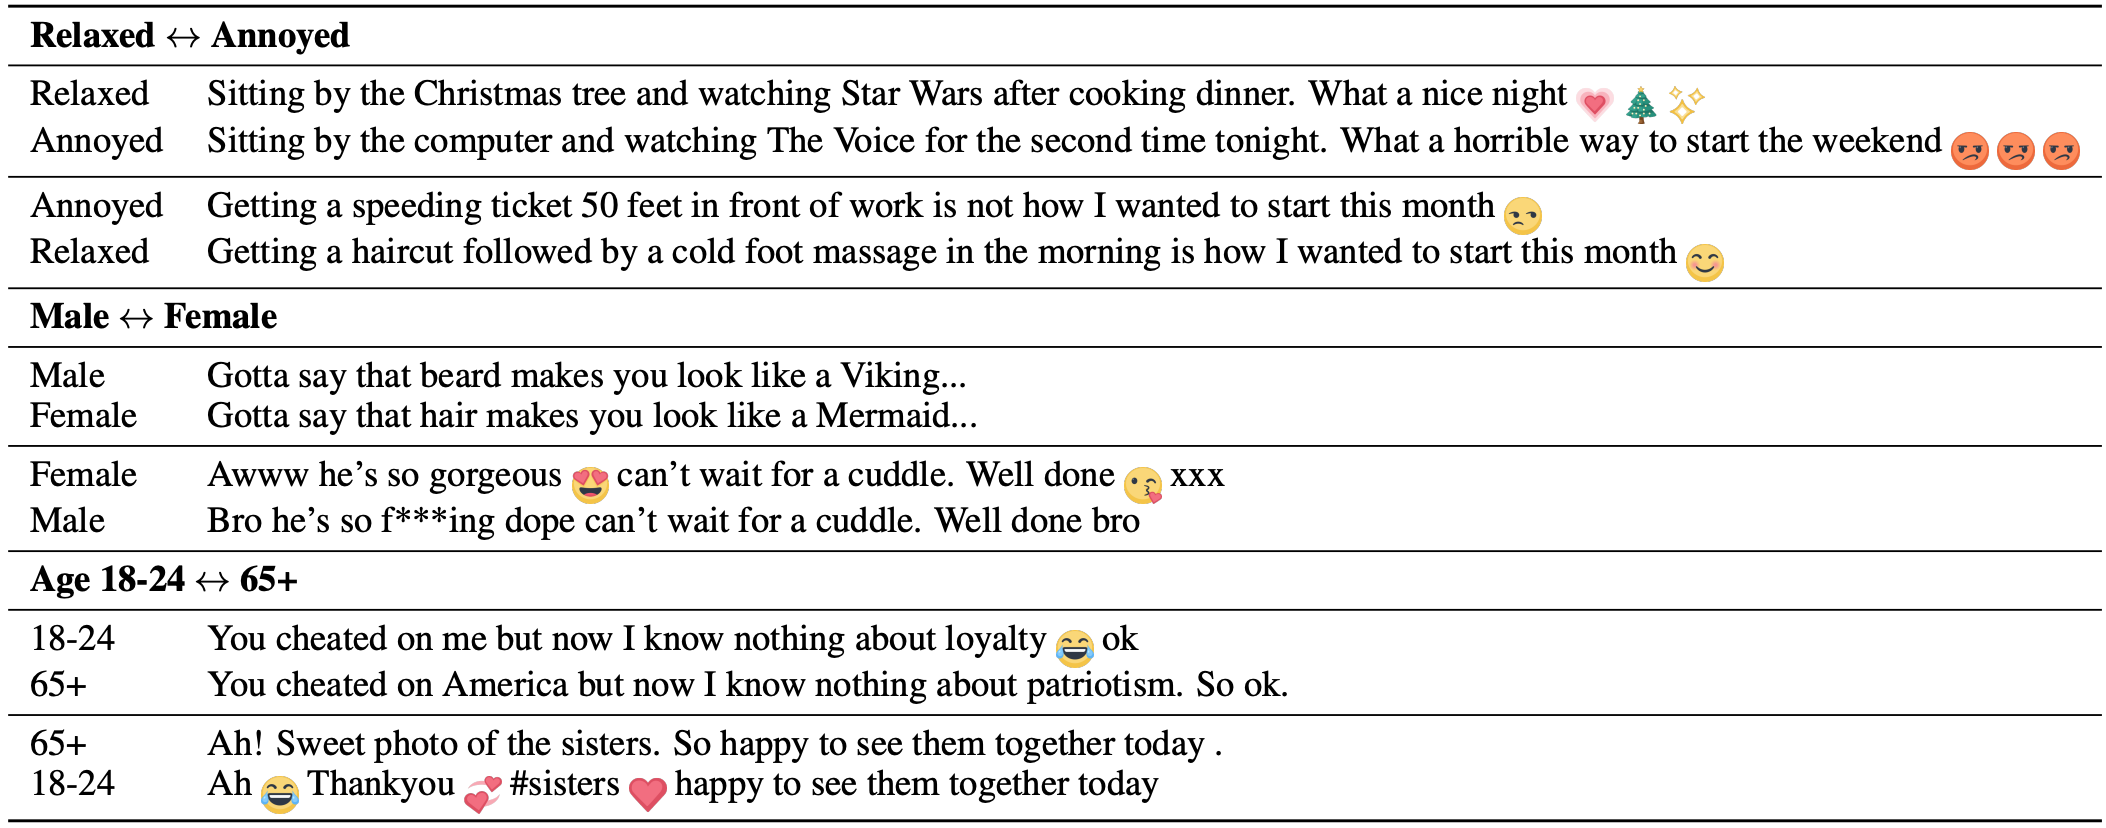
\includegraphics[width=\textwidth]{images/style-transfer-without-disentangling-samles}
\end{figure}
\end{frame}



\begin{frame}
\frametitle{Adversarial AutoEncoders (AAE)\footcite{AAE}}
VAE loss can be decomposed as:
\begin{equation*}
\begin{split}
%\expect[x \sim p_d(x)]{-\log p(x)} & \leq \expect[x]{\expect[q(z|x)]{-\log p(x | z)}} + \expect[x]{\kl{q(z|x)}{p(z)}} \\
%& = \expect[x]{\expect[q(z|x)]{-\log p(x | z)}} + \expect[x]{H() - H(q(z))} \\
\mathcal{L} = \expect[x]{\expect[q(z|x)]{\log p(x | z)}} + \expect[x]{H(q(z|x))} - CE(q(z) | p(z))
\end{split}
\end{equation*}
\begin{itemize}
    \item First term is a reconstruction loss, other two terms are regularization
    \item AAE replaces this regularization by training a GAN to distinguish samples from $q(z)$ and $p(z)$
    \item Encoder is deterministic (because quality is the same)
    \item To sample from $q(z)$ we sample $x \sim p_d(x)$ and then compute $z = E(x)$
\end{itemize}
\end{frame}


\begin{frame}
\frametitle{Adversarially Regularized Autoencoders (ARAE)\footcite{ARAE}}
\begin{itemize}
    \item ARAE is like AAE but now $p(z)$ is a generator (flexible prior!)
    \item How to transfer style with this thing? By disentangling:
    \begin{itemize}
        \item Train classifier to guess attributes in latent code
        \item Train encoder to spoof it (so, it's a GAN without real samples)
    \end{itemize}
    \item Flaws: sensitive to hyperparameters and have bad samples from prior\footcite{Sentence_generation_methods_comparison}
\end{itemize}

\begin{figure}
\centering
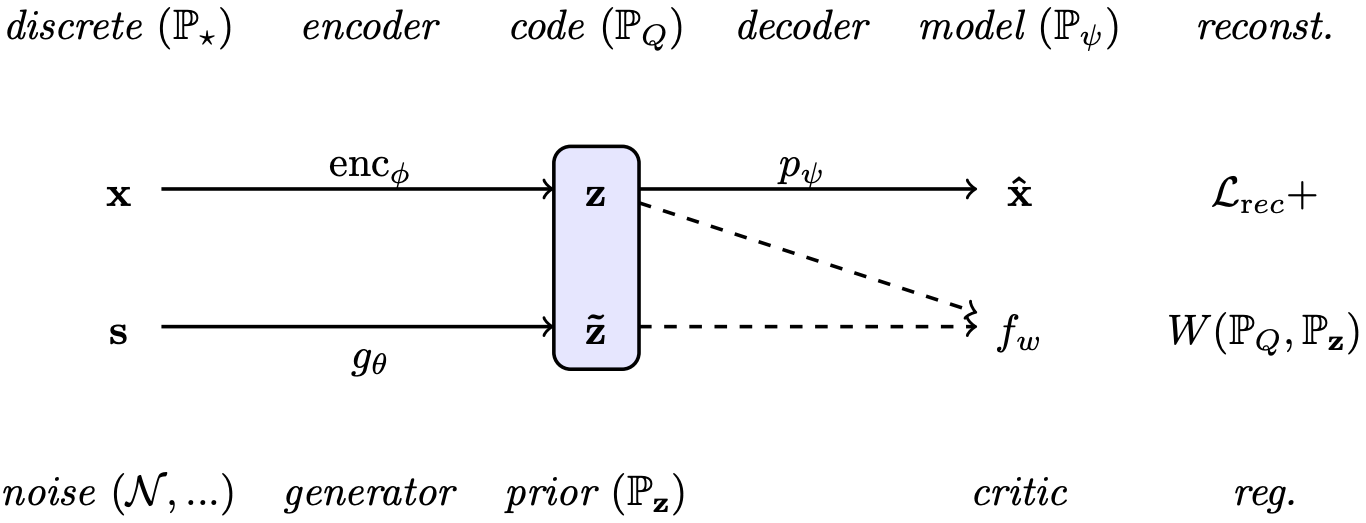
\includegraphics[width=0.8\textwidth]{images/arae}
\end{figure}

\end{frame}


\begin{frame}
\frametitle{Adversarially Regularized Autoencoders (ARAE)}
Samples from posterior:
\begin{figure}
\centering
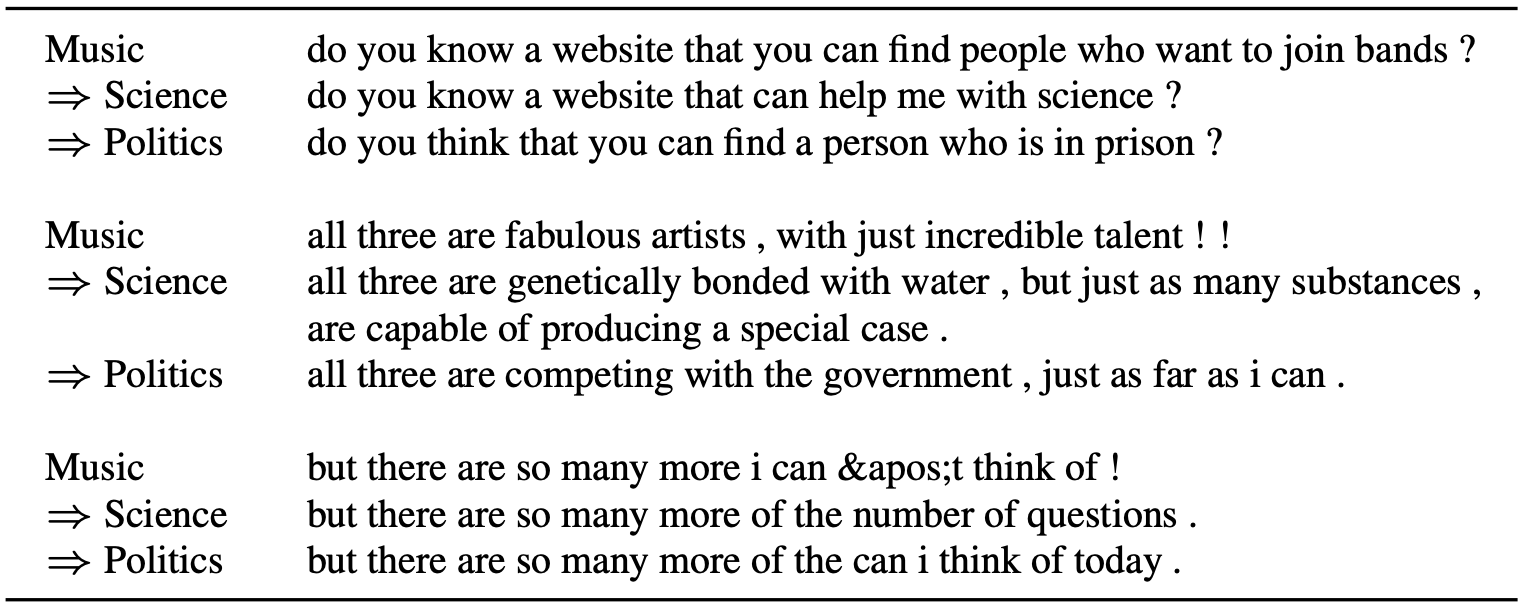
\includegraphics[width=0.8\textwidth]{images/arae-yahoo-samples}
\end{figure}

Samples from prior (without style transfer):
\begin{figure}
\centering
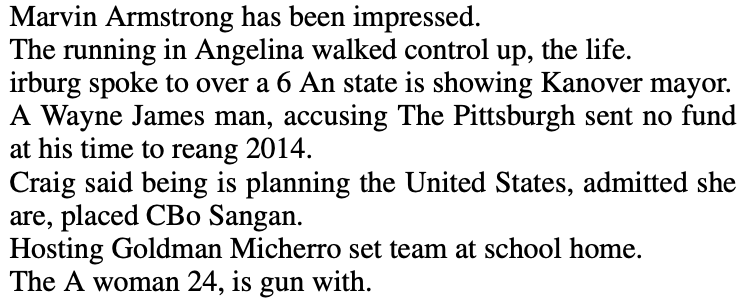
\includegraphics[width=0.5\textwidth]{images/arae-samples-from-prior}
\end{figure}
\end{frame}


%\begin{frame}
%\frametitle{Something like a summary}
%\begin{itemize}
%    \item Style Transfer in images is easy, in NLP we do not know
%\end{itemize}
%\end{frame}


\end{document}
